\chapter{Reliability Box Diagrams and Fault 
Tree Diagrams}
This chapter is based on
Refs.\cite{reliasoft}
and \cite{ftree-manual}.

In this chapter, we assume that
reader is familiar
with
Boolean Algebra. See 
 Chapter \ref{ch-conventions}
for a quick review 
of what
we recommend that you know about
Boolean Algebra
to fully appreciate this chapter.

\begin{figure}[h!]
\centering
\includegraphics[width=3in]
{reliability/relia-example.png}
\caption{Example of rbox diagram.} 
\label{fig-relia-rbox}
\end{figure}

\begin{figure}[h!]
\centering
\includegraphics[width=1.5in]
{reliability/relia-ftree.png}
\caption{An ftree diagram equivalent to
Fig.\ref{fig-relia-rbox}. It
represents 
$e=(\phi_1\A \phi_3)\V(\phi_2\A\phi_3)$. } 
\label{fig-relia-ftree}
\end{figure}

\begin{figure}[h!]
\centering
\includegraphics[width=3in]
{reliability/relia-map.png}
\caption{How to map an rbox diagram to a bnet.} 
\label{fig-relia-map}
\end{figure}

\begin{figure}[h!]
\centering
$$\xymatrix@-.5pc{
&\ul{\phi}_1\ar[d]&&\ul{\phi}_2\ar[d]
\\
&\rvx_1\ar[rr]
&&
\rvx_2
\ar `r[rd][rd]
\\
\rvb\ar`u[u][ru]
\ar`d[dr][rrd]
&&&&\rvA\ar[r]&\rve
\\
&&
\rvx_3
\ar `r[rru][rru]
\\
&&\ul{\phi}_3\ar[u]
}$$
\caption{bnet corresponding
the rbox diagram 
Fig.\ref{fig-relia-rbox}.}
\label{fig-relia-bnet}
\end{figure}

Complicated devices
with a large number 
of components
such as airplanes or rockets can
fail in many
ways. If
their performance
depends 
on some components
working in series
and one 
of the components
in the series
fails, this
may lead to
catastrophic failure.
To avert
such disasters,
engineers use equivalent
components
connected in parallel
instead of in series,
thus providing multiple backup
systems. They
analyze the
device to find its 
weak points and add
backup capabilities 
there. They also
estimate the
average time to failure
for the device. 



The two 
most popular diagrams
for finding the failure modes and their rates
for large complicated devices
are
\begin{itemize}
\item
rbox diagrams = Reliability Box diagrams. 
See Fig.\ref{fig-relia-rbox} for an example.
\item
ftree diagrams = Fault Tree Diagrams.
See Fig.\ref{fig-relia-ftree} for an example.
\end{itemize}
In an ftree diagram,
several nodes might
stand for the same 
component of a physical device.
In an rbox diagram,
on the
other hand, 
each node
represents a distinct  component
in a device. Hence, rbox diagrams
resemble the device they are
addressing
whereas ftree diagrams don't.
Henceforth, we will
refer to this desirable property
as {\bf  physical resemblance}.

As we will
show below with an example,
it is pretty
straightforward
to translate
an rbox to  an ftree diagram.
Going the other
way, translating
an ftree to an rbox diagram
is much more difficult.



Next we will define
a new kind of bnet
that we will call a failure bnet
that has physical resemblance.
Then we will describe
a simple method of translating (i.e., mapping)
any rbox diagram to a failure bnet.
Then we will show
how a failure
bnet can be used
to do all the
calculations
that are normally
done with an rbox
or an ftree diagram.
In that sense,
failure bnets
seem to afford
all the benefits
of both ftree and rbox 
diagrams.


A {\bf failure bnet} contains
nodes of 5  types,
labeled $\rvb$, $\rve$, $\rvx_i$,
$\ul{\phi}_i$, and $\rvA_i$.
All nodes have only
two possible states
$S=Success=0$, $F=Failure=1$.
\begin{enumerate}
\item 
The bnet has a beginning node labeled
$\rvb$ which is always set to success.
The $\rvb$ node
and the $\ul{\phi}_i$
nodes are the only root nodes of
the bnet.

\item The bnet has 
a single leaf node, the end node, labeled 
$\rve$. $\rve$ is fixed.
In rbox diagrams,
$\rve=S$
whereas in ftree diagrams, $\rve=F$.

\item
$\rvx^{nx}=
(\rvx_0, \rvx_1, \ldots, \rvx_{nx-1})$.
$\rvx_i\in \{S, F\}$ for all $i$.

Suppose $\rvx_i$
has parents 
$\ul{\phi}_i$ and $\rva^{na}=(\rva_0, \rva_1,
\dots \rva_{na-1})$.
Then the TPM of node $\rvx_i$ is
defined to be

 
\beq\color{blue}
P(x_i|\phi_i,a^{na})=
\delta(x_i,\phi_i\V  \V_{i=0}^{na-1} a_i)
\eeq

\item
For each node $\rvx_i$, the bnet has
 a ``performance"
 root node $\ul{\phi}_i\in \bool$
with an arrow
pointing from it 
to $\rvx_i$ (i.e, 
$\ul{\phi}_i\rarrow \rvx_i$).
For all $i$,

\beq \color{blue}
P(\phi_i)=
\eps_i \delta(\phi_i, F)
+\ol{\eps}_i\delta(\phi_i, S)
\;.
\eeq
$\eps_i$ is the failure probability
and $\ol{\eps}_i=1-\eps_i$
is the success probability.
We name the failure
probability $\eps_i$
because it
is normally very small.
It is usually
set to
$1-e^{-\lam_it}\approx \lam_it$
when $\lam_it<<1$,
where $\lam_i$
is the failure rate
for node $\rvx_i$
and $t$ stands for time.
The rblock
literature
usually calls 
$\ol{\eps_i}=R_i$
the {\bf reliability}
 of 
node $\rvx_i$,
and 
$\eps_i=(1-R_i)=F_i$
its {\bf unreliability}.


\item
The nodes $\rvA_i\in \bool$ 
are simply AND gates.
If $\rvA_i$ has inputs $\rvy^{ny}=
(\rvy_0, \rvy_1,
\ldots, \rvy_{ny-1})$,
then the TPM of $\rvA_i$ is

\beq\color{blue}
P(A_i|y^{ny})=
\delta(A_i, \A_{i=0}^{ny-1}y_i)
\;.
\eeq

\end{enumerate}

An instance (instantiation)
of a bnet is the bnet 
with all nodes set to
a specific state.
A {\bf realizable instance (r-instance)}
of a bnet is one
which has non-zero probability.

Fig.\ref{fig-relia-map}
shows how to translate
any rbox diagram
to a failure bnet.
To illustrate this procedure,
we translated the rbox diagram
Fig.\ref{fig-relia-rbox}
into the failure bnet 
Fig.\ref{fig-relia-bnet}.

For the
failure bnet 
Fig.\ref{fig-relia-bnet},
one has:

\beq
\begin{array}{l}\color{blue}
P(b)=\indi(b=0)\\\color{blue}
P(x_1|\phi_1, b)=\indi(x_1=\phi_1\V b)\\\color{blue}
P(x_2|\phi_2, x_1)=\indi(x_2=\phi_2\V x_1)\\\color{blue}
P(x_3|\phi_3, b)=\indi(x_3=\phi_3\V b)\\\color{blue}
P(A|x_2, x_3)e=\indi(x_2\A x_3)\\\color{blue}
P(e|A)=\indi(e=A)
\end{array}
\;.
\eeq
Therefore, all r-instances
of this bnet  must
satisfy

\beqa
e&=&(\phi_1\V\phi_2)\A \phi_3
\\
&=&(\phi_1\A \phi_3)\V(\phi_2\A\phi_3)
\;.
\label{eq-ftree}
\eeqa
Eq.(\ref{eq-ftree})
proves that 
Fig.\ref{fig-relia-ftree}
is indeed a 
representation 
of Fig.\ref{fig-relia-rbox}.

Next, we consider 
r-instances of this bnet for 
two cases: $e=S$ and $e=F$.

\begin{itemize}
\item {\bf rblock analysis: $e=S=0$.}\\
Table \ref{tab-probs-end-0}
shows the
probability of all possible r-instances
that end in success
for the failure bnet Fig.\ref{fig-relia-bnet}.
(These r-instances are
the main focus of rblock analysis).
The first 4 of
those probabilities (those with
$\phi_3=0$) sum to $\ol{\eps}_3$
so the sum $P(e=S)$ of all 
5 is

\beq
P(e=S)=\ol{\eps}_3
+ \ol{\eps}_1\ol{ \eps}_2 \eps_3
\;,
\eeq
or, expressing
it in reliability language
in which $\ol{\eps}=R$,

\beq
P(e=S)=R_3
+ R_1 R_2 \ol{R}_3
\;.
\eeq


% using array package and
%\begin{tabular}{|m{5cm}|m{2cm}|} for next table



% Please add the following required packages to your document preamble:
% \usepackage[table,xcdraw]{xcolor}
% If you use beamer only pass "xcolor=table" option, i.e., \documentclass[xcolor=table]{beamer}
\begin{table}[]
\centering
\begin{tabular}{|m{5cm}|m{2cm}|}
\hline
\rowcolor[HTML]{ECF4FF} 
instance & probability \\ \hline
$\rbd{0}{1}{0}{0}$ & $\ol{\eps}_1 \eps_2\ol{\eps}_3$ \\ \hline
$\rbd{1}{0}{0}{0}$ & $\eps_1 \ol{\eps}_2 \ol{\eps}_3$ \\ \hline
$\rbd{1}{1}{0}{0}$ & $\eps_1\eps_2\ol{\eps}_3$ \\ \hline
$\rbd{0}{0}{0}{0}$ & $\ol{\eps}_1 \ol{\eps}_2 \ol{\eps}_3$ \\ \hline
$\rbd{0}{0}{1}{0}$ & $\ol{\eps}_1\ol{\eps}_2\eps_3$ \\ \hline
\end{tabular}
\caption{Probabilities of all possible
 r-instances with $e=S=0$ for failure bnet
 Fig.\ref{fig-relia-bnet}.}
\label{tab-probs-end-0}
\end{table}


\item {\bf ftree analysis: $e=F=1$.}\\
Table \ref{tab-probs-end-1}
shows the
probability of all possible r-instances
that end in failure
for the failure bnet Fig.\ref{fig-relia-bnet}.
(These r-instances are
the main focus of ftree analysis).
If we set 
 $\eps_i=\eps$
and $\ol{\eps}_i\approx 1$
for $i=1,2,3$, then the first
two of those r-instances
have probabilities of $order(\eps^2)$
and the third has probability of
$order(\eps^3)$.
The two lowest order ($order(\eps^2)$)
r-instances
are called the ``minimal cut sets"
of the ftree. 
We will have more to say 
about minimal cut sets later on.
For now,
just note
from Eq.(\ref{eq-ftree})
that the ftree Fig.\ref{fig-relia-ftree}
is just the result
of joining
together with ORs
two expressions, one for each 
of the
two minimal cut sets.




% Please add the following required packages to your document preamble:
% \usepackage[table,xcdraw]{xcolor}
% If you use beamer only pass "xcolor=table" option, i.e., \documentclass[xcolor=table]{beamer}
\begin{table}[]
\centering
\begin{tabular}{|m{5cm}|m{2cm}|}
\hline
\rowcolor[HTML]{ECF4FF} 
instance & probability \\ \hline
$\rbd{0}{1}{1}{1}$ & $\ol{\eps}_1 \eps_2\eps_3$ \\ \hline
$\rbd{1}{0}{1}{1}$ & $\eps_1 \ol{\eps}_2 \eps_3$ \\ \hline
$\rbd{1}{1}{1}{1}$ & $\eps_1\eps_2\eps_3$ \\ \hline
\end{tabular}
\caption{Probabilities of all possible 
r-instances with $e=F=1$ for  the failure bnet
 Fig.\ref{fig-relia-bnet}.}
\label{tab-probs-end-1}
\end{table}

\end{itemize}

\hrule\noindent
{\bf More general $\rvx_i$.}\\
Failure bnets can actually
accommodate
$\rvx_i$ nodes
of a more general
kind than what we first stipulated.
Here are some possibilities: 



For any $a^n\in\bool^n$, let
\beq
len(a^n)=\sum_i a_i
\eeq

\begin{itemize}
\item {\bf OR gate}

\beqa\color{blue}
P(x_i|\phi_i,a^{na})&=&\color{blue}
\delta(x_i, \phi_i\V\V_j a_j)
\\
&=& \color{blue}
\delta(x_i, \phi_i\V\indi(len(a^{na})>0))
\eeqa

\item {\bf AND gate}

\beqa\color{blue}
P(x_i|\phi_i,a^{na})&=&\color{blue}
\delta(x_i, \phi_i\V\A_j a_j)
\\
&=& \color{blue}
\delta(x_i, \phi_i\V\indi(len(a^{na})=na))
\eeqa

\item {\bf Fail if least  $K$ failures
(less than $K$ successes)}

\beq\color{blue}
P(x_i|\phi_i,a^{na})=
\delta(x_i, \phi_i\V\indi(len(a^{na})\geq K))
\eeq

\item {\bf Fail if less than $K$ failures (at
least $K$ successes)}

\beq\color{blue}
P(x_i|\phi_i,a^{na})=
\delta(x_i, \phi_i\V\indi(len(a^{na})< K))
\eeq

\item {\bf Fail if exactly one failure}

\beq\color{blue}
P(x_i|\phi_i,a^{na})=
\delta(x_i, \phi_i\V\indi(len(a^{na})=1))
\eeq
This equals an XOR (exclusive OR)
gate when $na=2$.

\item {\bf General gate}\\
$f:\bool^{na}\rarrow \bool$

\beq\color{blue}
P(x_i|\phi_i,a^{na})=
\delta(x_i, \phi_i\V f(a^{na}))
\eeq
 
\end{itemize}
\hrule
\section{Minimal Cut Sets}

Suppose $x\in\bool$ and $f:\bool\rarrow \bool$.
Then
by direct evaluation, we see that

\beq
f(x)=[\ol{x}f(0)]\V [xf(1)]
\;.\label{eq-or-f}
\eeq
Let

\beq
\begin{array}{l}
!x=1-x,\\
!^0x=x,\\
!^1x=!x
\end{array}
\eeq
Then Eq.(\ref{eq-or-f})
can be rewritten as
 
\beq
f(x)= \V_{a\in\bool} [(!^{\ol{a}}x) f(a)]
\label{eq-ors-of-ands-1}
\;.
\eeq
Now suppose $x^n\in \bool^n$
and $f:\bool^n\rarrow \bool$.
Eq.(\ref{eq-ors-of-ands-1})
generalizes to

\beq
f(x^n)= \V_{a^n\in\bool^n}
 [\prod_i(!^{\ol{a}_i}x_i) f(a^n)]
\label{eq-ors-of-ands-n}
\;.
\eeq
Eq.(\ref{eq-ors-of-ands-n})
is called an {\bf ors-of-ands} normal form 
expansion.
There is also an {\bf ands-of-ors} normal
form expansion 
obtained by swapping multiplication
and $\V$
in Eq.(\ref{eq-ors-of-ands-n}), 
but we won't need it here.

A {\bf cut
set} is a set
of $\phi_i$'s such that
if they are all equal to $F$,
then $e=F$ for all the
r-instances.
A {\bf minimal cut set}
is a cut set such that there
are no larger cut sets that contain it.
From the failure bnet,
we can always find 
a function $f:\bool^{nx}\rarrow\bool$
such that
$e=f(\phi^{nx})$
for all the r-instances.
We did that for our
example failure
bnet and obtained Eq.(\ref{eq-ftree}).
We can
then
express 
$f(\phi^{nx})$ as an ors-of-ands expansion
to find all the minimal cut sets.
The ands
terms in that ors-of-ands
expansion 
each gives
a different minimal cut set,
after some simplification.
The ors-of-ands
expression
is not unique
and it may be necessary to simplify 
(using the Boolean Algebra identities
given in Chapter \ref{ch-conventions})
to remove those redundancies.